Para la siguiente sección, se buscó diseñar un puente que permita medir capacitores desde $100 \ nF$ hasta $1 \ \mu F$, trabajando a una frecuencia de $20 \ kHz$. Los capacitores a medir con dicho instrumento se caracterizan por poseer un factor de disipación D en un rango acotado entre $0.02$ y $0.12$.

Con lo dicho anteriormente, se tuvo que elegir entre tres posibles puentes: el serie, el paralelo y el de Schearing. Debido a que este último se emplea para capacitores con de muy bajas perdidas, es decir, con un $D \ < \ 10^{-3}$, mientras que el paralelo se utiliza para capacitores de altas perdidas, se optó por valerse de un puente serie, ya que este está destinado a ser empleado en un rango de perdidas similar al que requiere.

\begin{figure}[H]
\begin{center}
\begin{circuitikz}[european voltages]
	\draw (0,0) to[rmeterwa, t=V, label=$V_d$] ++(3,0) to[R, l=$R_4$] ++(0,-2) to[short] ++(-4,0) node[ocirc](-vg){};
	\draw (0,0) to[open] ++(3,0) node[circ, label=right:$V_b$](vb){};
	\draw (vb) to[open] ++(-3,0) node[circ, label=left:$V_a$](va){};
	\draw (0,0) to[vR, mirror, l=$R_3$] ++(0,-2);
	\draw (0,1.5) to[vR, mirror, l=$R_1$] (0,0);
	\draw (0,1.5) to[C, l_=$C_1$] ++(0,1.5) to[short] ++(3,0) to[C, l=$C_x$] ++(0,-1.5) to[R, l =$R_x$] ++(0,-1.5);
	\draw (0,3) to[short] ++(-1,0) node[ocirc](vg){};
	\draw (-vg) to[open, v^= $V_g$] (vg);
\end{circuitikz}
	\caption{Puente serie implementado}
	\label{fig:puenteserie}
\end{center}
\end{figure}
Realizando los divisores resistivos para calcular la diferencia de potencial $V_d = V_a -V_b$:
\begin{align*}
	V_d=\frac{R_3}{R_3+R_1+\frac{1}{sC_1}}-\frac{R_4}{R_4+R_x+\frac{1}{sC_x}}
\end{align*}
Se realizó el análisis de sensibilidades para la tensión $Vd$, observando su variación en funcion de $R_1$ y $R_3$:
\begin{align*}
\scalebox{1.5}{$
S_{R_1}^{V_d} = \frac{\partial V_d}{\partial R_1} \cdot \frac{R_1}{V_d}=
\frac{-R_1R_3}{\left( \frac{R_3}{R_3+\frac{1}{sC_1}+R1}-\frac{R_4}{R_4+\frac{1}{sC_x}+R_x} \right) \cdot  \left( R_3+\frac{1}{sC_1}+R1\right)^2}
$}
\end{align*}

\begin{align*}
\scalebox{1.5}{$
S_{R_3}^{V_d} = \frac{\partial V_d}{\partial R_3} \cdot \frac{R_3}{V_d}=\frac{(C_1R_1s+1)R_3C_1(C_xR_xs+R_4C_xs+1)}{(C_1R_1s+C_1R_3s+1)\cdot (-C_1C_xR_3R_xs+R_4C_1C_xR_1s-C_1R_3+R_4C_x)}
$}
\end{align*}
Luego, mediante el análisis de sensibilidades, considerando los valores máximos y mínimos de capacitores y estableciendo $C_1 = 1 \ nF$ y $R_1 = 100 \ \Omega$, se obtienen los siguientes valores para los demás componentes:

\begin{equation*}
\begin{split}
	R_{1_{Min}} =& \ \frac{5 \cdot 10^{-7}}{\pi C_1} = 159 \ \Omega \\
	R_{1_{Max}} =& \ \frac{3 \cdot 10^{-6}}{\pi C_1} = 1 \ k\Omega \\
	R_{3_{Min}} =& \ \frac{R_4 \cdot 10^{-7}}{\pi C_1} = 10 \ k\Omega \\
	R_{3_{Max}} =& \ \frac{R_4 \cdot 10^{-6}}{\pi C_1} = 100 \ k\Omega
\end{split}
\end{equation*}



A continuación se  graficó la tensión del puente en función de las resistencias previamente mencionadas para una frecuencia.
\begin{figure}[H]
	\centering
	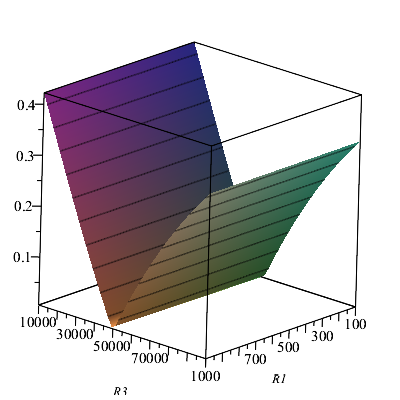
\includegraphics[width=0.4\textwidth]{/ImagenesEjercicio3/Graph.png}
	\caption{Tensión del puente en función de $R_1$ y $R_3$.}
	\label{fig:graph1}
\end{figure}

También se realizó una simulación de Montecarlo para asegurar que el puente converja al equilibrio.
\begin{figure}[H]
	\centering
	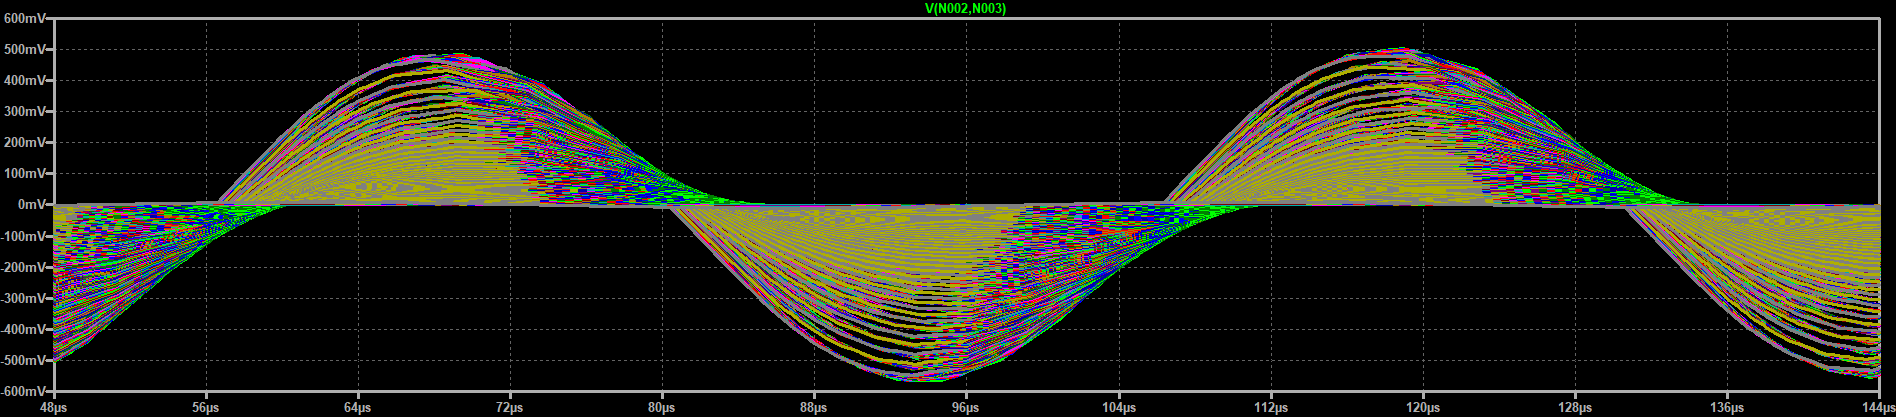
\includegraphics[width=\textwidth]{/ImagenesEjercicio3/Montecarlos.png}
	\caption{Diagramas de Montecarlo.}	
	\label{fig:graph2}
\end{figure}

Planteando la tensión en el equilibrio, y despejando algebraicamente, se llega a las siguientes expresiones:
\begin{equation*}
\begin{split}
	C_{x} =& \ \frac{C_1R_3}{R_4}\ F \\
	R_{x} =& \ \frac{R_1R_4}{R_3}\ \Omega \\
	D_{x} =& \ 2\pi f C_1R_1 
\end{split}
\end{equation*}

A partir de estas, se puede calcular la precisión del puente para estos parámetros:
\begin{equation*}
\begin{split}
	\Delta C_{x} =& \ \frac{C_1 \cdot \Delta R_3}{R_4}\  \\
	\Delta R_{x} =& \ \frac{\Delta R_1 \cdot R_4  R_3+R_1  R_4 \cdot \Delta R_3}{(R_3)^2}\  \\
	\Delta D_{x} =& \ 2\pi f C_1 \Delta R_1 
\end{split}
\end{equation*}

Obteniendo para cada capacitor una medición del punto de estabilización del puente.

% Please add the following required packages to your document preamble:
% \usepackage{multirow}
\begin{table}[H]
\hspace*{-1.5cm}
\scalebox{0.57}{
\centering
\begin{tabular}{|c|c|c|c|c|c|c|c|c|c|c|c|c|c|c|c|c|c|c|c|}
\hline
\multirow{2}{*}{\textit{Valor nominal}} & \multicolumn{6}{c|}{2 KHz}                       & \multicolumn{6}{c|}{20 KHz}                      & \multicolumn{6}{c|}{200 KHz}                  & \multirow{2}{*}{Observaciones}                                                                                                                 \\ \cline{2-19}
                                        & C       & D     & $\phi$ & C       & D & $\phi$ & C       & D     & $\phi$ & C       & D & $\phi$ & C      & D     & $\phi$ & C     & D & $\phi$ &                                                                                                                                                \\ \hline
100 nF                                   & 99.83 nF & 0.012 & -89.98      & 102 nF   & 0.01 & -84.99     & 114.1 nF & 0.022 & -89.85      & 101 nF   & 0.02 & -88.61      & 98.9 nF & 0.016 & -88.64      & 120 nF & 0.012 & -88.7      & -                                                                                                                                              \\ \hline
500 nF                                   & 507 nF   & 0.015     & -89.98     & 494.6 nF & 0.05 & -89.96      & 507 nF   & 0.02     & -89.87      & 514.6 nF & 0.23 & -88.55      & 530 nF  & 0.018     & -89.97      & 540 nF & 1 & -87.86      & -                                                                                                                                              \\ \hline
1 $\mu$F                                     & 1 $\mu$F     & 0.01     & -89.4      & 1 $\mu$F     & 0.15 & -82.22      & 1 $\mu$F     & 0.01     & -89.49      & 1 $\mu$F     & 0.022 & -87.84      & 1 $\mu$F    & 0.026     & -88.12      & 1 $\mu$F   & 0.023 & -86.97      & -                                                                                                                                              \\ \hline
2 $\mu$F                                     & 1 $\mu$F     & 0.03     & -89.12     & 1 $\mu$F     & 0.06 & -88.19     & 1 $\mu$F     & 0.019     & -89.49      & 1 $\mu$F     & 0.019 & -89.51      & 1 $\mu$F    & 0.035     & -88.48      & 1 $\mu$F   & 0.032 & -88.77      & \begin{tabular}[c]{@{}c@{}}El puente no llega al equilibrio\\  dado que se encuentra fuera del rango \\ para el cual fue diseñado\end{tabular} \\ \hline
\end{tabular}
}
\caption{Mediciones con el puente.}
\end{table}
%%%%%%%%%%%%100 NANO
\begin{figure}[H]
	\centering
	\includegraphics[width=0.4\textwidth,trim={0 2.2cm 0.1cm 1.75cm},clip]{/Mediciones/minimo/1xxnD0.x/2kHz.png}
	\includegraphics[width=0.4\textwidth,trim={0 2.2cm 0.1cm 1.75cm},clip]{/Mediciones/minimo/100nD0.02/2kHz.png}
	\subcaption{Medición de 100 nF a 2 kHz con distinto D [Derecha 0.012].}
	\label{fig:fcon1}
\end{figure}
\begin{figure}[H]
	\centering
	\includegraphics[width=0.4\textwidth,trim={0 2.2cm 0.1cm 1.75cm},clip]{/Mediciones/minimo/1xxnD0.x/20kHz.png}
	\includegraphics[width=0.4\textwidth,trim={0 2.2cm 0.1cm 1.75cm},clip]{/Mediciones/minimo/100nD0.02/20kHz.png}
\caption{Medición de 100 nF a 20 kHz con distinto D [Derecha 0.012].}
	\label{fig:fcon2}
\end{figure}
\begin{figure}[H]
	\centering
	\includegraphics[width=0.4\textwidth,trim={0 2.2cm 0.1cm 1.75cm},clip]{/Mediciones/minimo/1xxnD0.x/200kHz.png}
	\includegraphics[width=0.4\textwidth,trim={0 2.2cm 0.1cm 1.75cm},clip]{/Mediciones/minimo/100nD0.02/200kHz.png}
\caption{Medición de 100 nF a 200 kHz con distinto D [Derecha 0.012].}
	\label{fig:fcon3}
\end{figure}
%%%%%%%%%%%%500 nano
\begin{figure}[H]
	\centering
	\includegraphics[width=0.4\textwidth,trim={0 2.2cm 0.1cm 1.75cm},clip]{/Mediciones/media/4xxD0.x/2kHz.png}
	\includegraphics[width=0.4\textwidth,trim={0 2.2cm 0.1cm 1.75cm},clip]{/Mediciones/media/406nD0.02/2kHz.png}
\caption{Medición de 500 nF a 2 kHz con distinto D [Derecha 0.012].}
	\label{fig:fcon4}
\end{figure}
\begin{figure}[H]
	\centering
	\includegraphics[width=0.4\textwidth,trim={0 2.2cm 0.1cm 1.75cm},clip]{/Mediciones/media/4xxD0.x/20kHz.png}
	\includegraphics[width=0.4\textwidth,trim={0 2.2cm 0.1cm 1.75cm},clip]{/Mediciones/media/406nD0.02/20kHz.png}
\caption{Medición de 500 nF a 20 kHz con distinto D [Derecha 0.012].}
	\label{fig:fcon5}
\end{figure}
\begin{figure}[H]
	\centering
	\includegraphics[width=0.4\textwidth,trim={0 2.2cm 0.1cm 1.75cm},clip]{/Mediciones/media/4xxD0.x/200kHz.png}
	\includegraphics[width=0.4\textwidth,trim={0 2.2cm 0.1cm 1.75cm},clip]{/Mediciones/media/406nD0.02/200kHz.png}
\caption{Medición de 500 nF a 200 kHz con distinto D [Derecha 0.012].}
	\label{fig:fcon6}
\end{figure}
%%%%%%%%%%%%1 micro
\begin{figure}[H]
	\centering
	\includegraphics[width=0.4\textwidth,trim={0 2.2cm 0.1cm 1.75cm},clip]{/Mediciones/maximo/1xud0.x/2kHz.png}
	\includegraphics[width=0.4\textwidth,trim={0 2.2cm 0.1cm 1.75cm},clip]{/Mediciones/maximo/1ud0.2/2kHz.png}
\caption{Medición de 1 $\mu$F a 2 kHz con distinto D [Derecha 0.012].}
	\label{fig:fcon7}
\end{figure}
\begin{figure}[H]
	\centering
	\includegraphics[width=0.4\textwidth,trim={0 2.2cm 0.1cm 1.75cm},clip]{/Mediciones/maximo/1xud0.x/20kHz.png}
	\includegraphics[width=0.4\textwidth,trim={0 2.2cm 0.1cm 1.75cm},clip]{/Mediciones/maximo/1ud0.2/20kHz.png}
\caption{Medición de 1 $\mu$F a 20 kHz con distinto D [Derecha 0.012].}
	\label{fig:fcon8}
\end{figure}
\begin{figure}[H]
	\centering
	\includegraphics[width=0.4\textwidth,trim={0 2.2cm 0.1cm 1.75cm},clip]{/Mediciones/maximo/1xud0.x/200kHz.png}
	\includegraphics[width=0.4\textwidth,trim={0 2.2cm 0.1cm 1.75cm},clip]{/Mediciones/maximo/1ud0.2/200kHz.png}
\caption{Medición de 1 $\mu$F a 200 kHz con distinto D [Derecha 0.012].}
	\label{fig:fcon9}
\end{figure}
%%%%%%%%%%%%%2 micro
\begin{figure}[H]
	\centering
	\includegraphics[width=0.4\textwidth,trim={0 2.2cm 0.1cm 1.75cm},clip]{/Mediciones/doblemaximo/2xud0.x/2kHz.png}
	\includegraphics[width=0.4\textwidth,trim={0 2.2cm 0.1cm 1.75cm},clip]{/Mediciones/doblemaximo/2ud0.2/2kHz.png}
\caption{Medición de 2 $\mu$F a 2 kHz con distinto D [Derecha 0.012].}
	\label{fig:fcon10}
\end{figure}
\begin{figure}[H]
	\centering
	\includegraphics[width=0.4\textwidth,trim={0 2.2cm 0.1cm 1.75cm},clip]{/Mediciones/doblemaximo/2xud0.x/20kHz.png}
	\includegraphics[width=0.4\textwidth,trim={0 2.2cm 0.1cm 1.75cm},clip]{/Mediciones/doblemaximo/2ud0.2/20kHz.png}
\caption{Medición de 2 $\mu$F a 20 kHz con distinto D [Derecha 0.012].}
	\label{fig:fcon11}
\end{figure}
\begin{figure}[H]
	\centering
	\includegraphics[width=0.4\textwidth,trim={0 2.2cm 0.1cm 1.75cm},clip]{/Mediciones/doblemaximo/2xud0.x/200kHz.png}
	\includegraphics[width=0.4\textwidth,trim={0 2.2cm 0.1cm 1.75cm},clip]{/Mediciones/doblemaximo/2ud0.2/200kHz.png}
\caption{Medición de 2 $\mu$F a 200 kHz con distinto D [Derecha 0.012].}
	\label{fig:fcon12}
\end{figure}

Finalmente se realizaron las mismas mediciones en el analizador de impedancias para obtener un calculo del error, obteniendo las siguientes mediciones.\\
% Please add the following required packages to your document preamble:
% \usepackage{multirow}
\begin{table}[H]
\hspace*{-0.75cm}
\scalebox{0.65}{
\centering
\begin{tabular}{|c|c|c|c|c|c|c|c|c|c|c|c|c|c|c|c|c|c|c|}
\hline
\multirow{2}{*}{\textit{Valor nominal}} & \multicolumn{6}{c|}{2 KHz}                                     & \multicolumn{6}{c|}{20 KHz}                                   & \multicolumn{6}{c|}{200 KHz}                                 \\ \cline{2-19} 
                                        & C            & D     & $\phi$ & C             & D     & $\phi$ & C            & D     & $\phi$ & C            & D     & $\phi$ & C           & D     & $\phi$ & C            & D     & $\phi$ \\ \hline
100 nF                                  & 98.2 nF      & 0.017 & -89.03 & 98.5 nF       & 0.098 & -84.39 & 95.7 nF      & 0.016 & -89.03 & 94.8 nF      & 0.023 & -88.68 & 92 nF       & 0.02  & -88.81 & 91 nF        & 0.017 & -89.03 \\ \hline
500 nF                                  & 434 nF       & 0.02  & -88.44 & 453 nF        & 0.062 & -86.36 & 387 nF       & 0.015 & -89.14 & 406 nF       & 0.019 & -88.92 & 402 nF      & 0.022 & -88.76 & 415 nF       & 0.026 & -88.5  \\ \hline
1 $\mu F$                               & 1 $\mu F$    & 0.01  & -89.39 & 0.9 $\mu F$   & 0.124 & -82.9  & 0.97 $\mu F$ & 0.008 & -89.54 & 0.76 $\mu F$ & 0.02  & -88.5  & 1 $\mu F$   & 0.03  & -88    & 0.74 $\mu F$ & 0.035 & -88    \\ \hline
2 $\mu F$                               & 1.71 $\mu F$ & 0.027 & -88.43 & 1.872 $\mu F$ & 0.059 & -86.55 & 1.5 $\mu F$  & 0.014 & -89.22 & 1.74 $\mu F$ & 0.015 & -89.17 & 1.5 $\mu F$ & 0.04  & -87.8  & 1.8 $\mu F$  & 0.04  & -87.7  \\ \hline
\end{tabular}
}
\caption{Mediciones con el analizador de impedancias.}
\end{table}

Luego, comparando los valores obtenidos en ambas tablas y analizando el peor caso, se puede aproximar el error del puente, siendo este:
\begin{equation*}
\begin{split}
	 Error \% =& \ \frac{|C_{Gen}-C_{Puente}|}{C_{Puente}} \approx 15 \% 
\end{split}
\end{equation*}

Finalmente, se puede concluir que el error porcentual obtenido puede reducirse utilizando un amplificador de instrumentación que permita medir la tensión $V_d$, permitiendo calibrar los presets con mayor precisión. Otra forma de mejorar las mediciones es utilizando mayor cantidad de presets, garantizando que estos sean de distinta magnitud. De esta forma, se puede obtener un menor paso con los de menor impedancia, de la misma forma que se realizó en el inciso anterior.